%%%%
%%%%  FIGURE
%%%%
%\begin{landscape}
\begin{figure}[ht] 
\vbox{\vspace{-1cm}
\centering
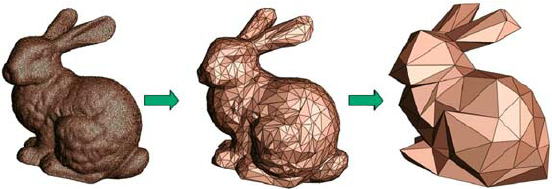
\includegraphics[width=.72\textwidth]{./Pics/Introduction/Graphical-illustration-of-model-order-reduction.png}
\vspace{0.cm}
\vspace{0.5cm}
}   
\caption{Graphical illustration of model order reduction (initially used by \citet{Schilders2008}, with graphics credited to Harvard University, Microsoft Research.)}
\vspace{1.5cm}
\label{fig:IllustrationMOR}
\end{figure}

\begin{figure}[ht] 
\vbox{\vspace{-1cm}
\centering
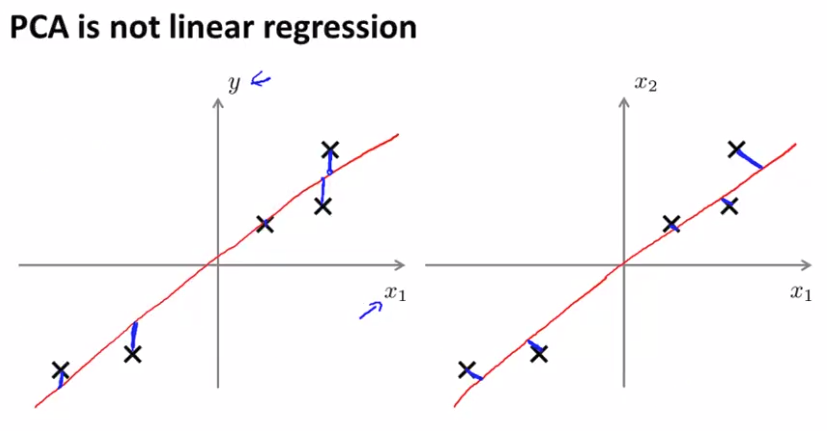
\includegraphics[width=.72\textwidth]{./Pics/PCA_LinReg/PCA_is_not_LinReg.png}
\vspace{0.cm}
\hbox{\hspace{0.25cm} (a) Linear regression \hspace{2cm} (b) PCA \hspace{3.0cm}}
\vspace{0.5cm}
}   
\caption{Graphical comparision between linear regression and PCA (extracted from \citet{AndrewNg_2018})}
\vspace{1.5cm}
\label{fig:PCA_is_not_LinReg}
\end{figure}
%\end{landscape}
\clearpage

%%%%
%%%%  FIGURE
%%%%
%\begin{landscape}
\begin{figure}[ht] 
\vbox{\vspace{-1cm}
\hbox{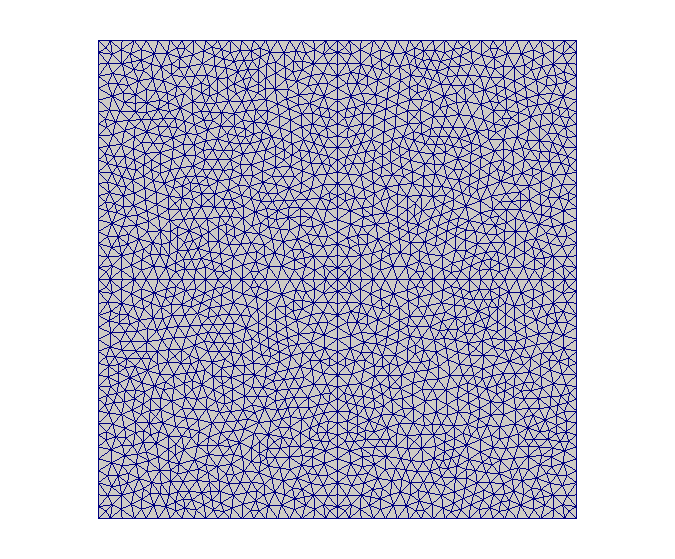
\includegraphics[width=.56\textwidth]{./Pics/BaseCase/BaseCase_MeshOnly.png}
      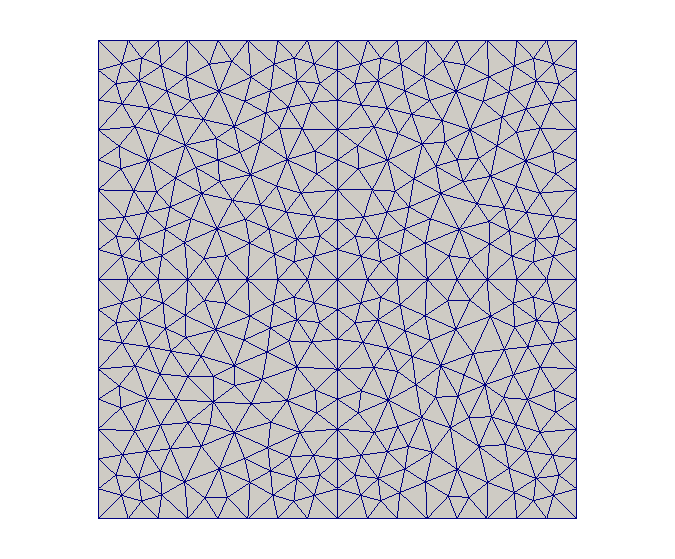
\includegraphics[width=.56\textwidth]{./Pics/ArithMeanCase/ArithMeanCase_MeshOnly.png}}
\vspace{0.cm}
\hbox{\hspace{0.25cm} (a) High Resolution Grid (BaseCase) \hspace{0.75cm} (b) Low Resolution Grid (Upscaled Cases) \hspace{3.0cm}}
\vspace{0.5cm}
}   
\caption{Mesh grid used in the performed numerical simulations: (a) high-resolution and (b) upscaled cases with 4112 and 728 triangular elements respectively}
\label{fig:HiRes_LowRes_Mesh}
\end{figure}
%\end{landscape}
\clearpage


%%%%
%%%%  FIGURE
%%%%
\begin{landscape}
\begin{figure}[ht] 
\vbox{\vspace{-1cm}
\hspace{0.0cm} \hbox{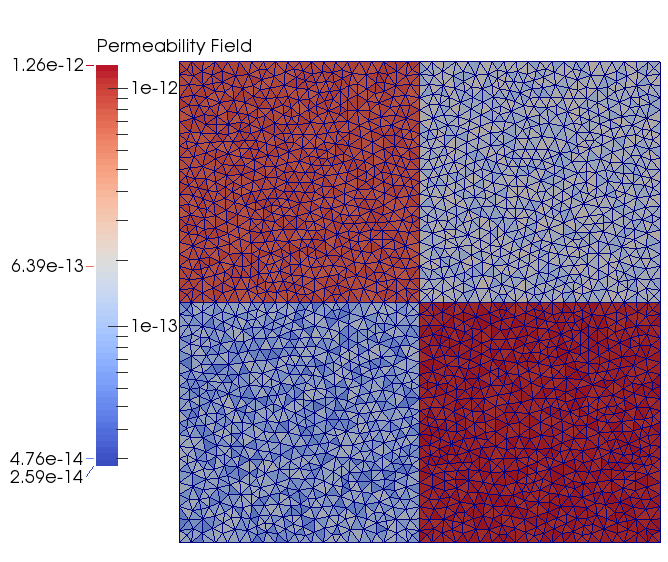
\includegraphics[width=.56\textwidth]{./Pics/BaseCase/BaseCase_PermField_withMesh.png}
      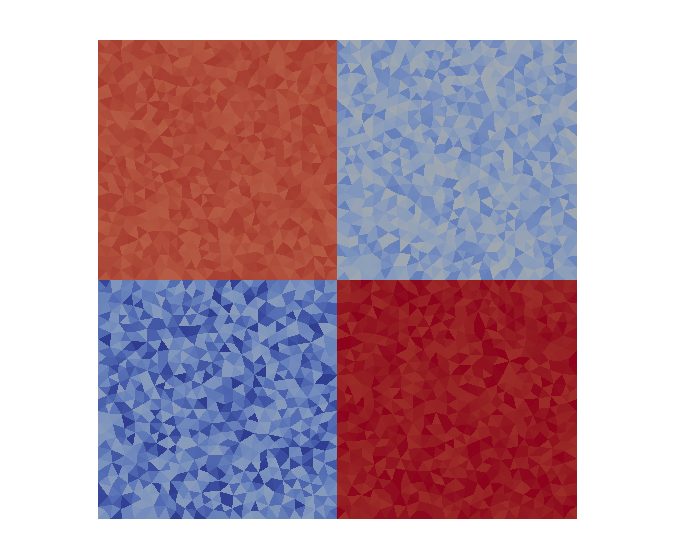
\includegraphics[width=.56\textwidth]{./Pics/BaseCase/BaseCase_PermField_withoutMesh2.png}
      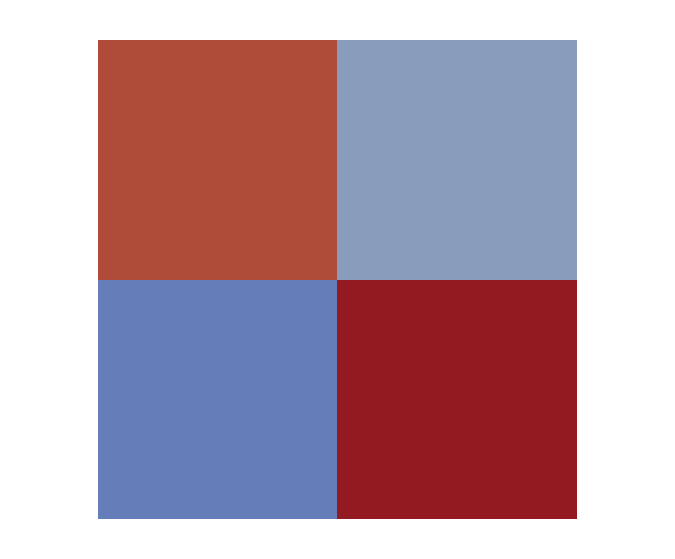
\includegraphics[width=.56\textwidth]{./Pics/ArithMeanCase/ArithMeanCase_PermField_withoutMesh2.png}}
\vspace{0.cm}
\hbox{\hspace{0.5cm} (a) BaseCase (overlapped with the mesh) \hspace{1.0cm} (b) BaseCase (without Mesh) \hspace{3.0cm} (c) ArithMean Case}
\vspace{0.5cm}
\hbox{
      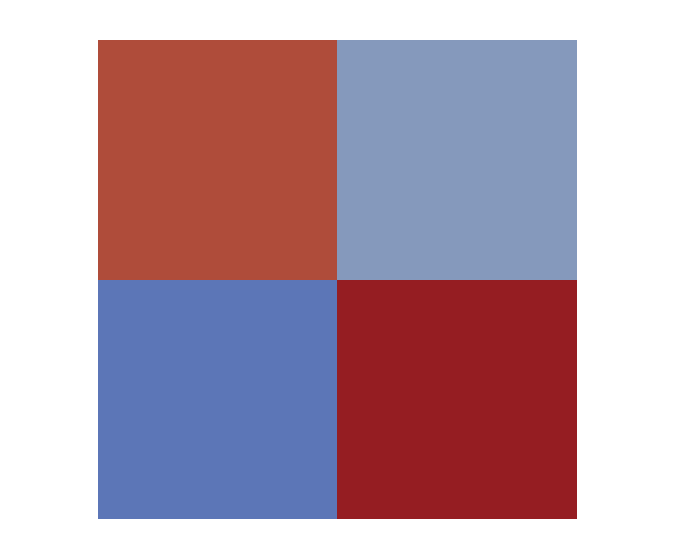
\includegraphics[width=.56\textwidth]{./Pics/HarmMeanCase/HarmMeanCase_PermField_withoutMesh2.png}
      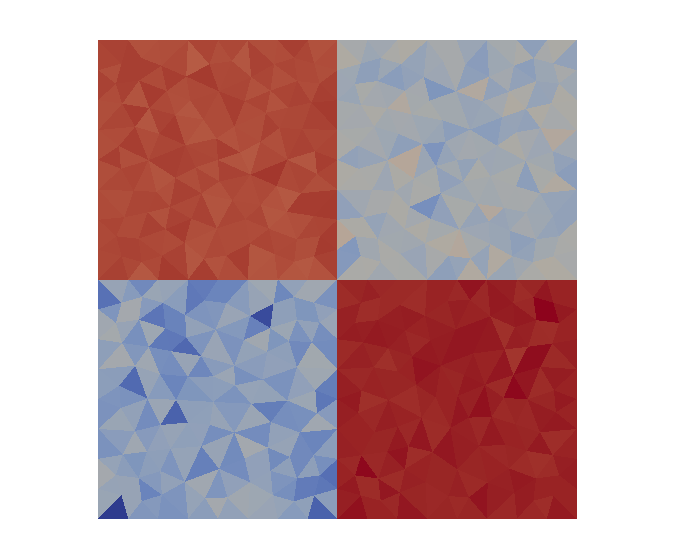
\includegraphics[width=.56\textwidth]{./Pics/PDFCase/PDFCase_PermField_withoutMesh2.png} 
      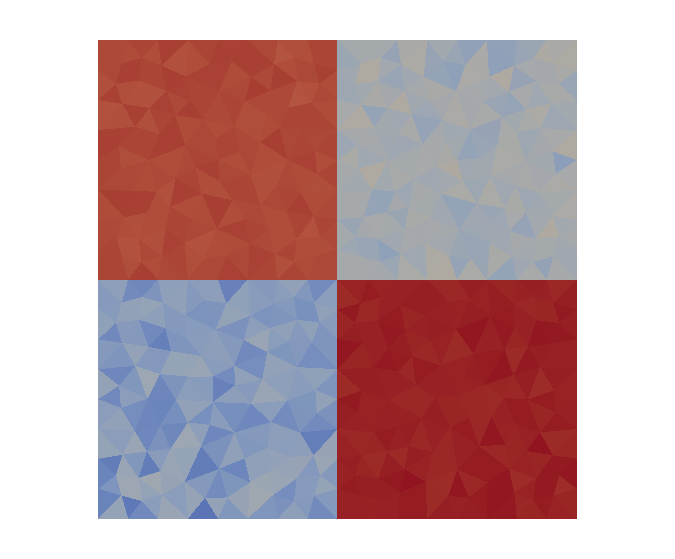
\includegraphics[width=.56\textwidth]{./Pics/SVDCase/SVDCase_PermField_withoutMesh2.png}}
\vspace{0.cm}
\hbox{ \hspace{1.5cm} (d) HarmMean Case \hspace{4.75cm} (e) PDFCase  \hspace{5.0cm} (f) SVDCase}
\vspace{0.cm}
}   
\caption{Permeability field for the base case as well as the upscaled cases (Permeability legend in Fig.~\ref{fig:PermFields}(a) is representative for all the other figures - \ie Fig.~\ref{fig:PermFields}(b) to (f))}
\label{fig:PermFields}
\end{figure}
\end{landscape}
\clearpage


%%%%
%%%%  FIGURE
%%%%
\begin{landscape}
\begin{figure}[ht] 
\vbox{\vspace{-1cm}
\hspace{0.0cm} \hbox{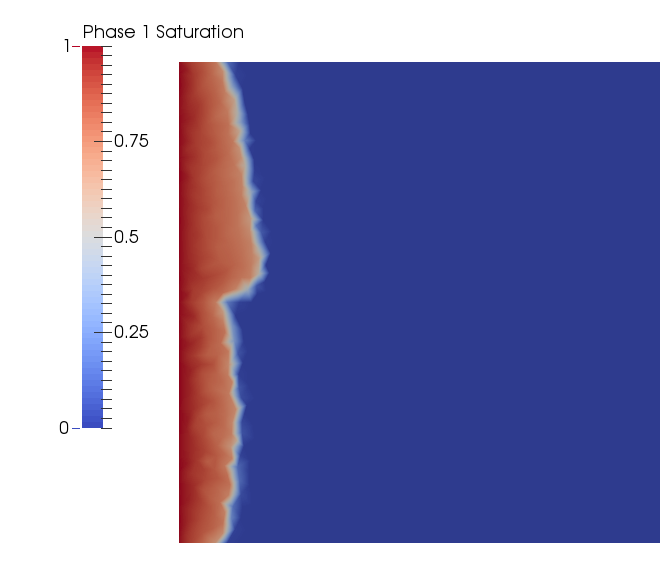
\includegraphics[width=.56\textwidth]{./Pics/BaseCase/BaseCase_Saturation_t_dot15.png}
      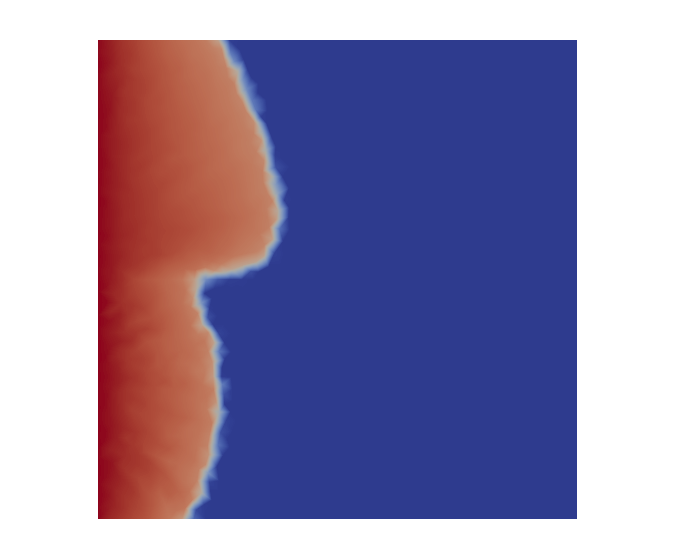
\includegraphics[width=.56\textwidth]{./Pics/BaseCase/BaseCase_Saturation_t_dot30.png}
      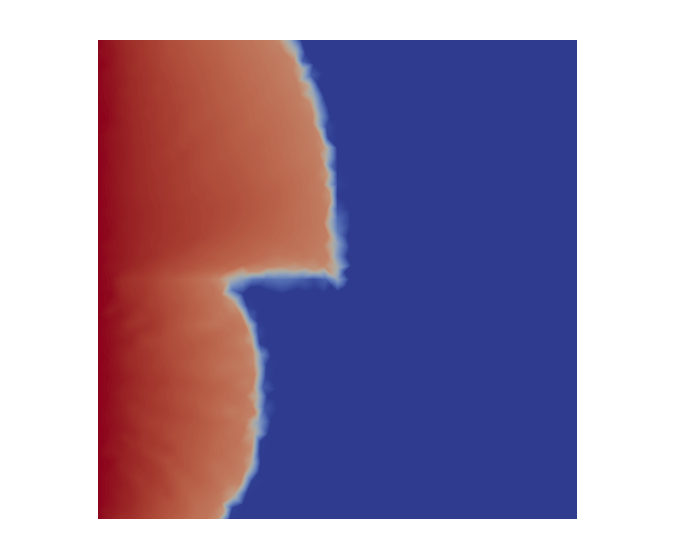
\includegraphics[width=.56\textwidth]{./Pics/BaseCase/BaseCase_Saturation_t_dot50.png}}
\vspace{0.cm}
\hbox{\hspace{0.5cm} (a) Phase 1 Saturation at t=0.15s \hspace{3.75cm} (b) t=0.30s \hspace{5.0cm} (c) t=0.50s}
\vspace{0.5cm}
\hbox{
      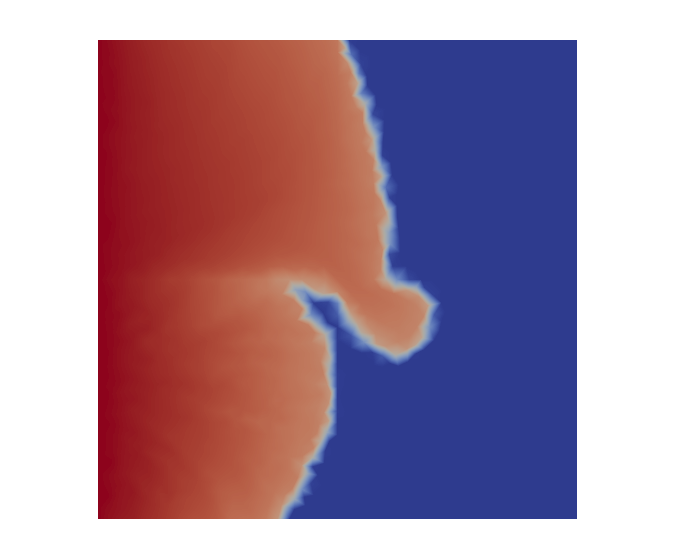
\includegraphics[width=.56\textwidth]{./Pics/BaseCase/BaseCase_Saturation_t_1dot15.png}
      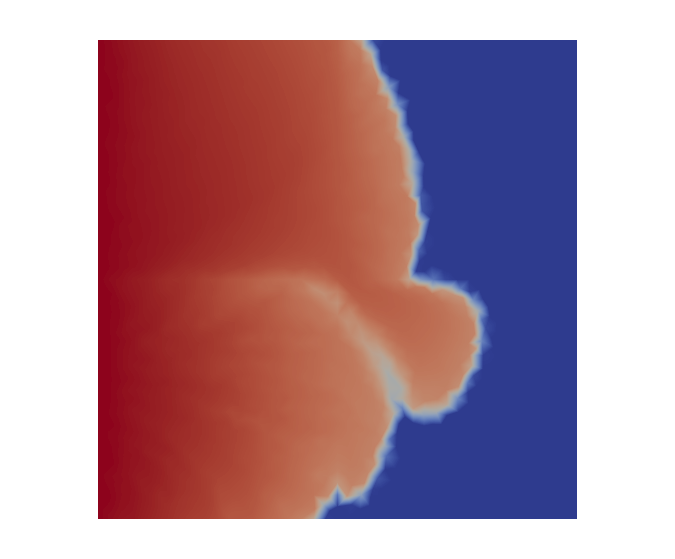
\includegraphics[width=.56\textwidth]{./Pics/BaseCase/BaseCase_Saturation_t_1dot75.png} 
      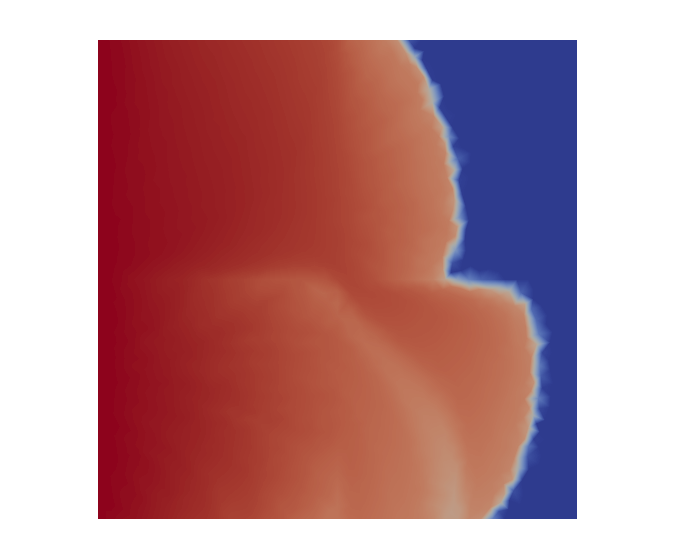
\includegraphics[width=.56\textwidth]{./Pics/BaseCase/BaseCase_Saturation_t_2dot95.png}}
\vspace{0.cm}
\hbox{ \hspace{2.5cm} (d) t=1.15s \hspace{5.5cm} (e) t=1.75s   \hspace{5.5cm} (f) t=2.95s}
\vspace{0.cm}
}   
\caption{Simulations for the BaseCase (Saturation legend in Fig.~\ref{fig:BaseCase_Saturation}(a) is representative for all the other figures - \ie Fig.~\ref{fig:BaseCase_Saturation}(b) to (f))}
\label{fig:BaseCase_Saturation}
\end{figure}
\end{landscape}
\clearpage


%%%%
%%%%  FIGURE
%%%%
\begin{landscape}
\begin{figure}[ht] 
\vbox{\vspace{-1cm}
\hspace{0.0cm} \hbox{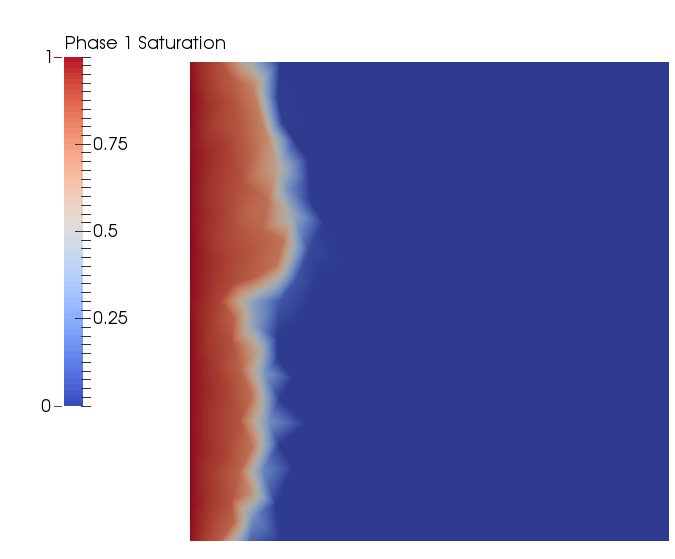
\includegraphics[width=.56\textwidth]{./Pics/ArithMeanCase/ArithMeanCase_Saturation_t_dot15.png}
      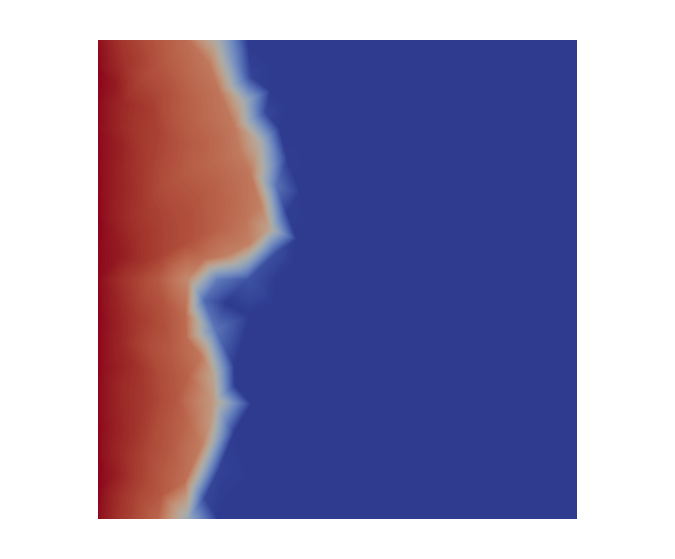
\includegraphics[width=.56\textwidth]{./Pics/ArithMeanCase/ArithMeanCase_Saturation_t_dot30.png}
      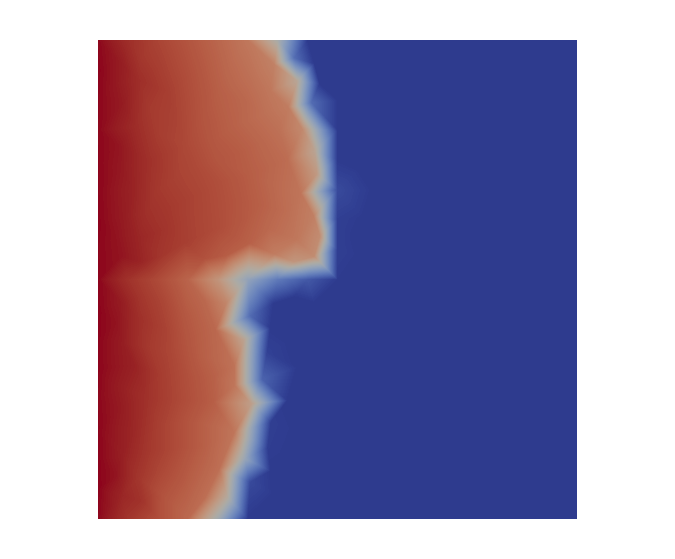
\includegraphics[width=.56\textwidth]{./Pics/ArithMeanCase/ArithMeanCase_Saturation_t_dot50.png}}
\vspace{0.cm}
\hbox{\hspace{0.5cm} (a) Phase 1 Saturation at t=0.15s \hspace{3.75cm} (b) t=0.30s \hspace{5.0cm} (c) t=0.50s}
\vspace{0.5cm}
\hbox{
      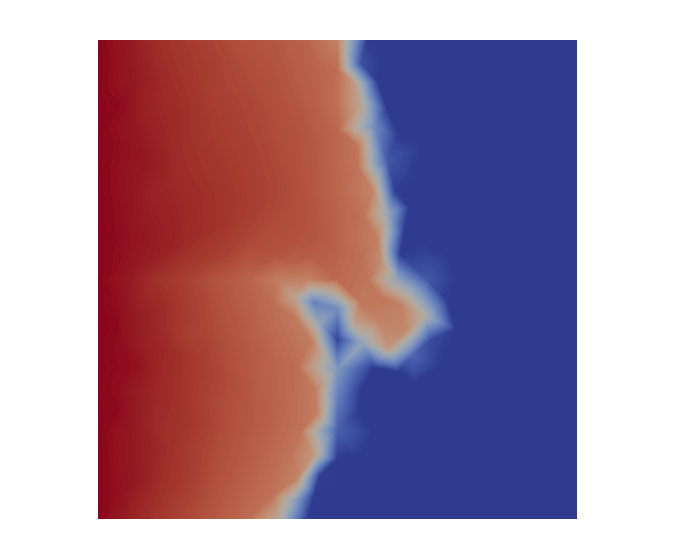
\includegraphics[width=.56\textwidth]{./Pics/ArithMeanCase/ArithMeanCase_Saturation_t_1dot15.png}
      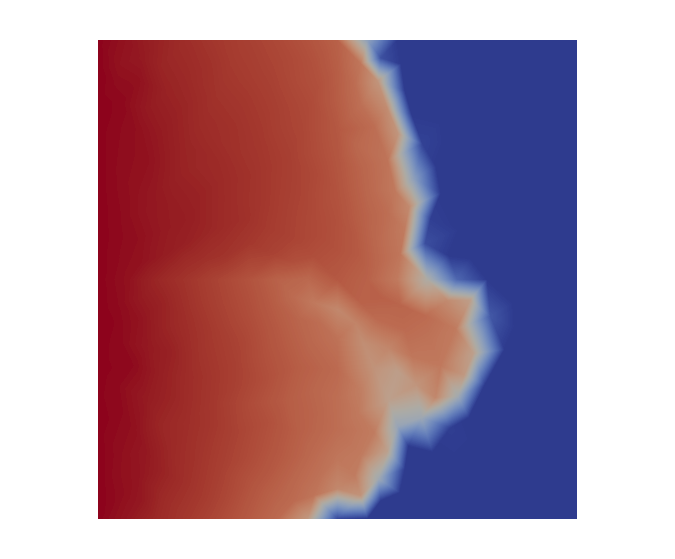
\includegraphics[width=.56\textwidth]{./Pics/ArithMeanCase/ArithMeanCase_Saturation_t_1dot75.png} 
      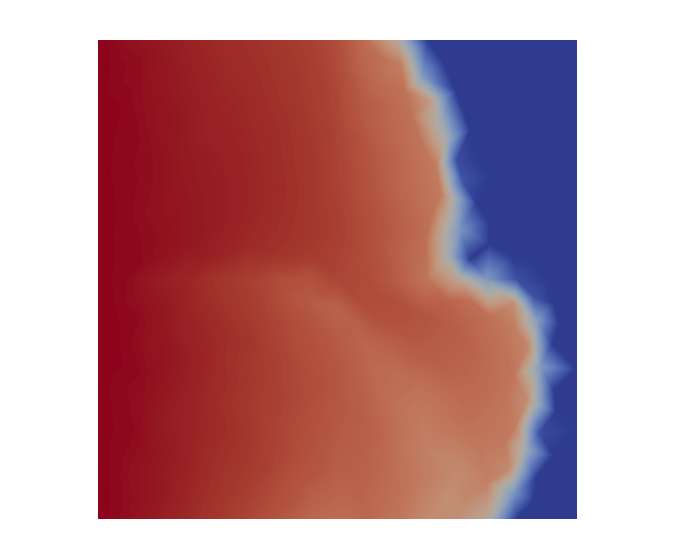
\includegraphics[width=.56\textwidth]{./Pics/ArithMeanCase/ArithMeanCase_Saturation_t_2dot95.png}}
\vspace{0.cm}
\hbox{ \hspace{2.5cm} (d) t=1.15s \hspace{5.5cm} (e) t=1.75s   \hspace{5.5cm} (f) t=2.95s}
\vspace{0.cm}
}   
\caption{Simulations for the ArithMean Case (Saturation legend in Fig.~\ref{fig:ArithMeanCase_Saturation}(a) is representative for all the other figures - \ie Fig.~\ref{fig:ArithMeanCase_Saturation}(b) to (f))}
\label{fig:ArithMeanCase_Saturation}
\end{figure}
\end{landscape}
\clearpage



%%%%
%%%%  FIGURE
%%%%
\begin{landscape}
\begin{figure}[ht] 
\vbox{\vspace{-1cm}
\hspace{0.0cm} \hbox{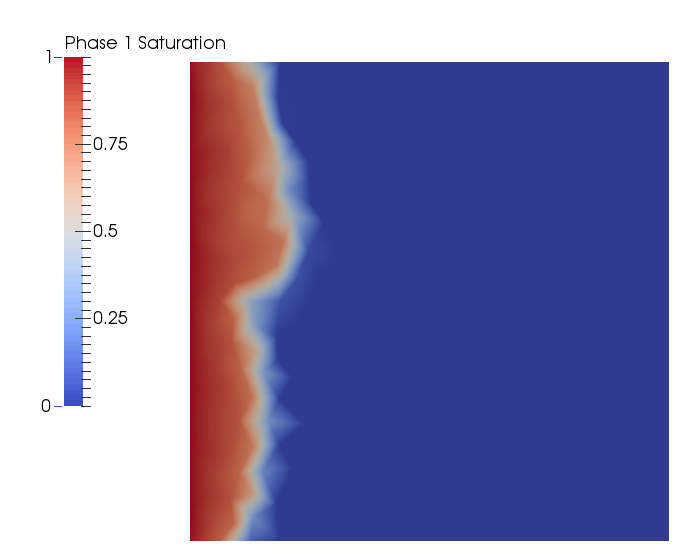
\includegraphics[width=.56\textwidth]{./Pics/HarmMeanCase/HarmMeanCase_Saturation_t_dot15.png}
      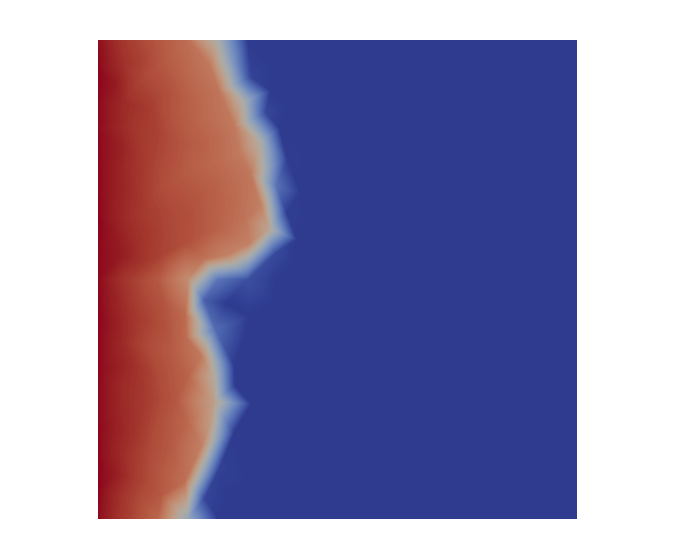
\includegraphics[width=.56\textwidth]{./Pics/HarmMeanCase/HarmMeanCase_Saturation_t_dot30.png}
      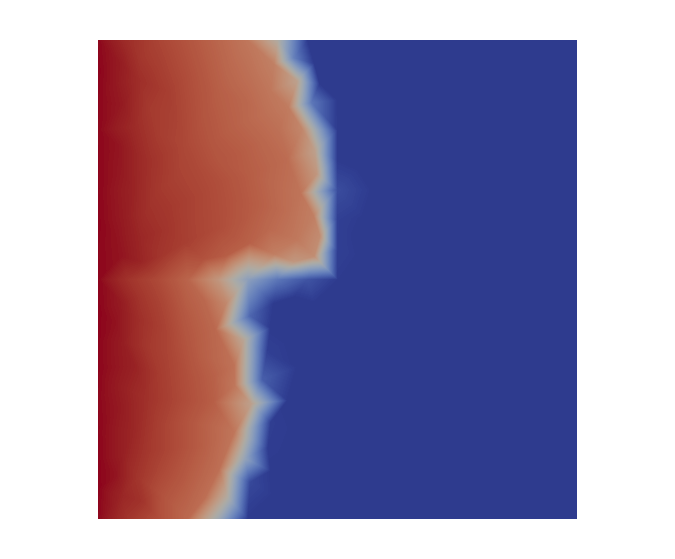
\includegraphics[width=.56\textwidth]{./Pics/HarmMeanCase/HarmMeanCase_Saturation_t_dot50.png}}
\vspace{0.cm}
\hbox{\hspace{0.5cm} (a) Phase 1 Saturation at t=0.15s \hspace{3.75cm} (b) t=0.30s \hspace{5.0cm} (c) t=0.50s}
\vspace{0.5cm}
\hbox{
      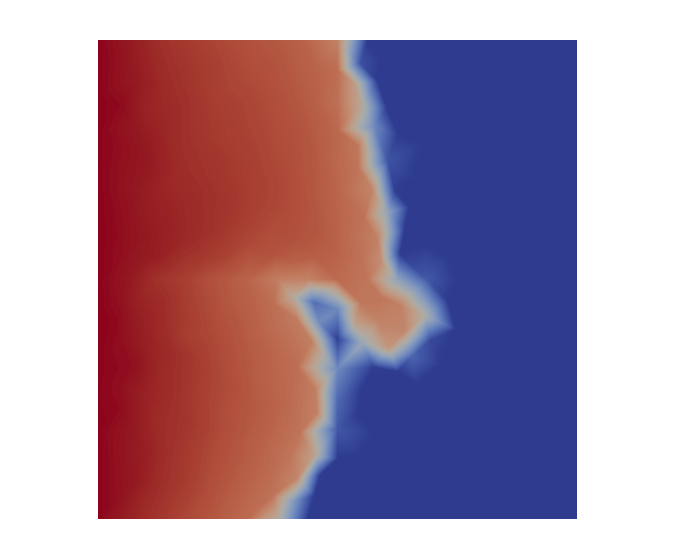
\includegraphics[width=.56\textwidth]{./Pics/HarmMeanCase/HarmMeanCase_Saturation_t_1dot15.png}
      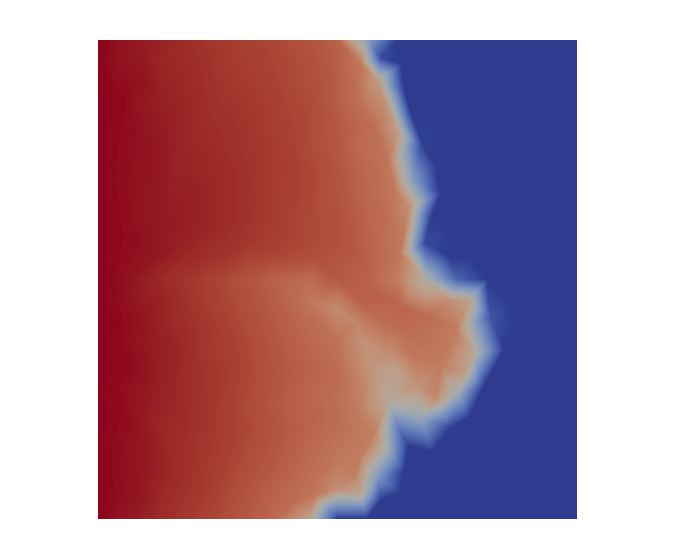
\includegraphics[width=.56\textwidth]{./Pics/HarmMeanCase/HarmMeanCase_Saturation_t_1dot75.png} 
      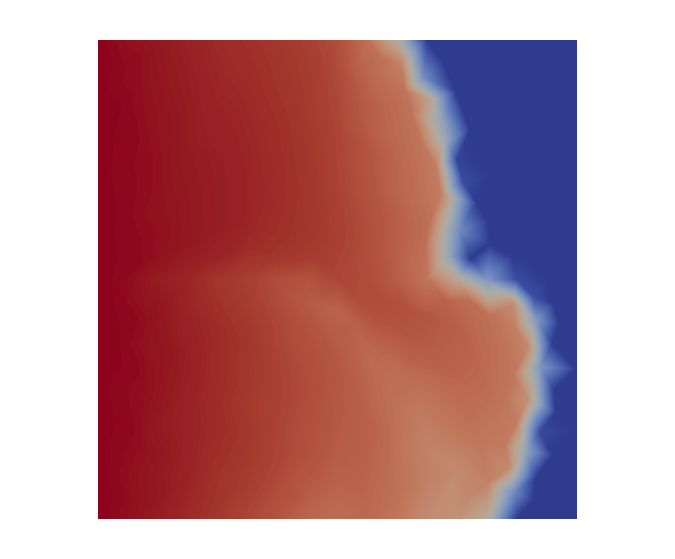
\includegraphics[width=.56\textwidth]{./Pics/HarmMeanCase/HarmMeanCase_Saturation_t_2dot95.png}}
\vspace{0.cm}
\hbox{ \hspace{2.5cm} (d) t=1.15s \hspace{5.5cm} (e) t=1.75s   \hspace{5.5cm} (f) t=2.95s}
\vspace{0.cm}
}   
\caption{Simulations for the HarmMean Case (Saturation legend in Fig.~\ref{fig:HarmMeanCase_Saturation}(a) is representative for all the other figures - \ie Fig.~\ref{fig:HarmMeanCase_Saturation}(b) to (f))}
\label{fig:HarmMeanCase_Saturation}
\end{figure}
\end{landscape}
\clearpage





%%%%
%%%%  FIGURE
%%%%
\begin{landscape}
\begin{figure}[ht] 
\vbox{\vspace{-1cm}
\hspace{0.0cm} \hbox{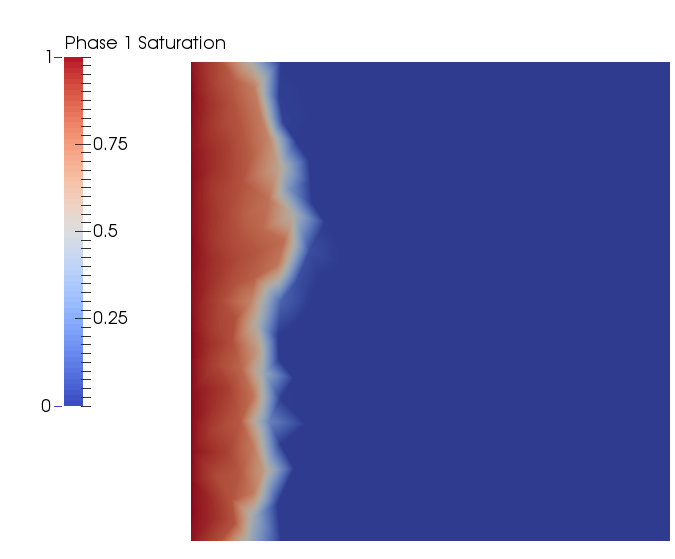
\includegraphics[width=.56\textwidth]{./Pics/PDFCase/PDFCase_Saturation_t_dot15.png}
      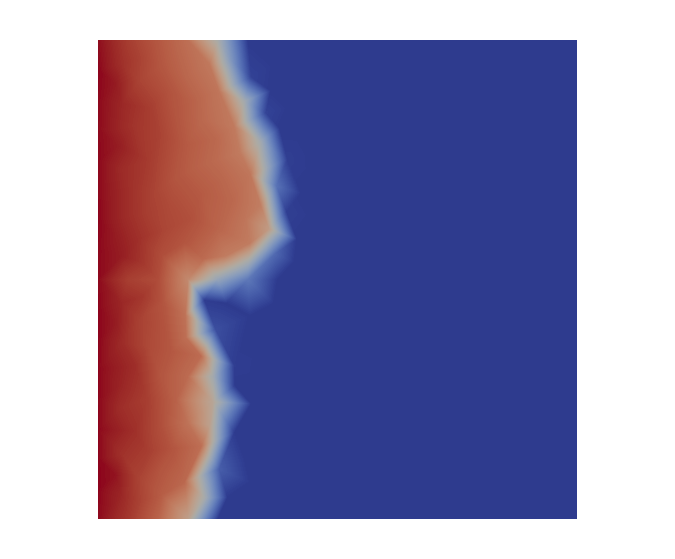
\includegraphics[width=.56\textwidth]{./Pics/PDFCase/PDFCase_Saturation_t_dot30.png}
      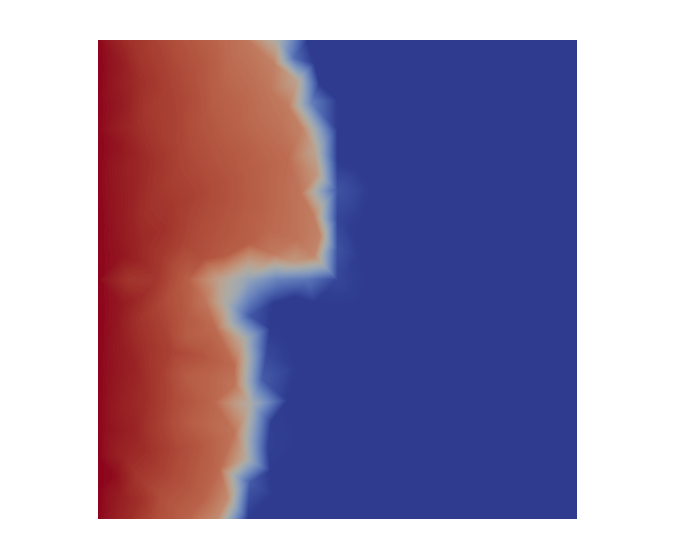
\includegraphics[width=.56\textwidth]{./Pics/PDFCase/PDFCase_Saturation_t_dot50.png}}
\vspace{0.cm}
\hbox{\hspace{0.5cm} (a) Phase 1 Saturation at t=0.15s \hspace{3.75cm} (b) t=0.30s \hspace{5.0cm} (c) t=0.50s}
\vspace{0.5cm}
\hbox{
      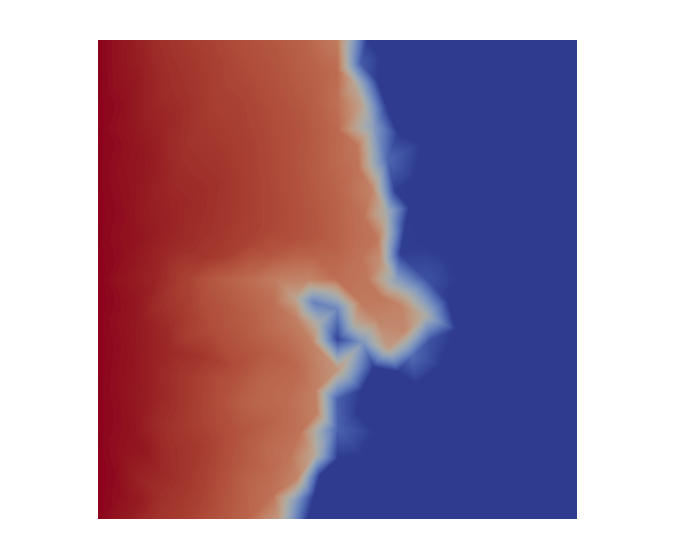
\includegraphics[width=.56\textwidth]{./Pics/PDFCase/PDFCase_Saturation_t_1dot15.png}
      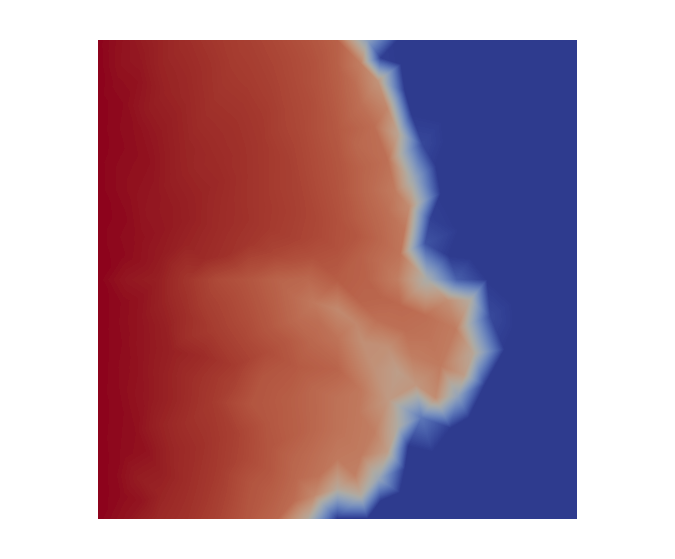
\includegraphics[width=.56\textwidth]{./Pics/PDFCase/PDFCase_Saturation_t_1dot75.png} 
      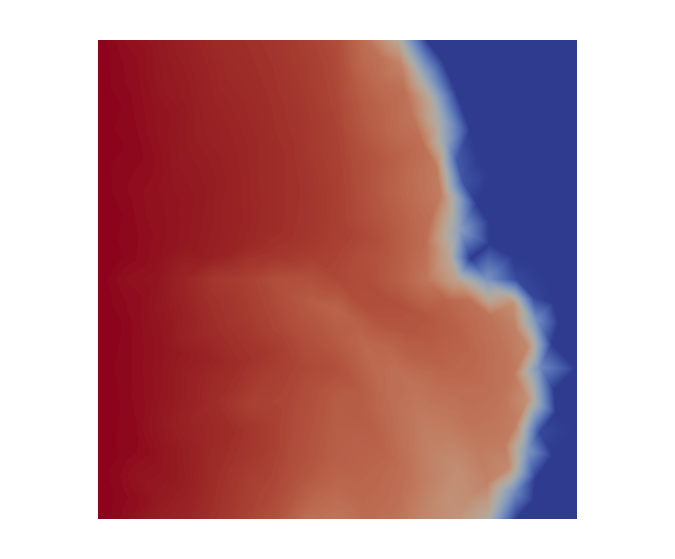
\includegraphics[width=.56\textwidth]{./Pics/PDFCase/PDFCase_Saturation_t_2dot95.png}}
\vspace{0.cm}
\hbox{ \hspace{2.5cm} (d) t=1.15s \hspace{5.5cm} (e) t=1.75s   \hspace{5.5cm} (f) t=2.95s}
\vspace{0.cm}
}   
\caption{Simulations for the PDFCase (Saturation legend in Fig.~\ref{fig:PDFCase_Saturation}(a) is representative for all the other figures - \ie Fig.~\ref{fig:PDFCase_Saturation}(b) to (f))}
\label{fig:PDFCase_Saturation}
\end{figure}
\end{landscape}
\clearpage



%%%%
%%%%  FIGURE
%%%%
\begin{landscape}
\begin{figure}[ht] 
\vbox{\vspace{-1cm}
\hspace{0.0cm} \hbox{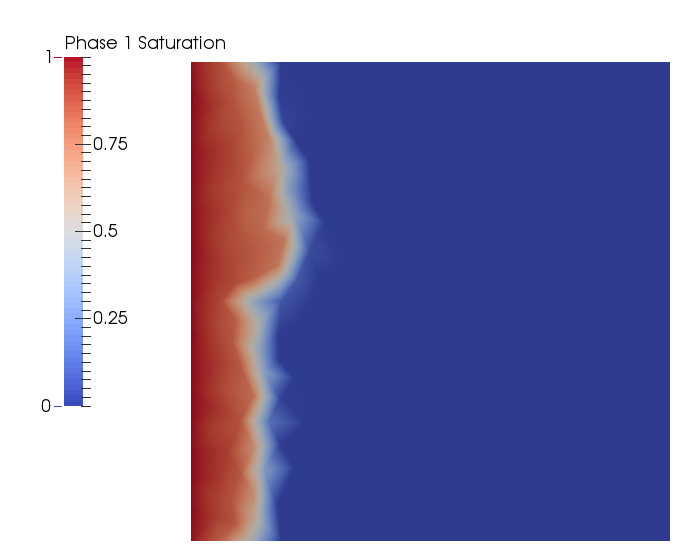
\includegraphics[width=.56\textwidth]{./Pics/SVDCase/SVDCase_Saturation_t_dot15.png}
      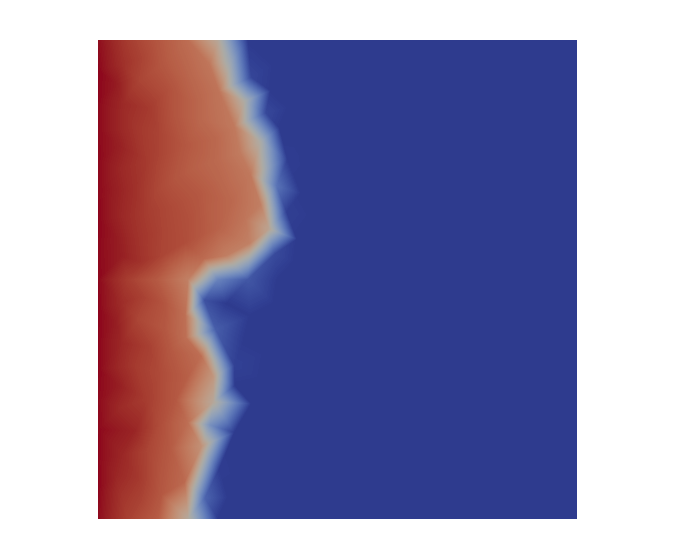
\includegraphics[width=.56\textwidth]{./Pics/SVDCase/SVDCase_Saturation_t_dot30.png}
      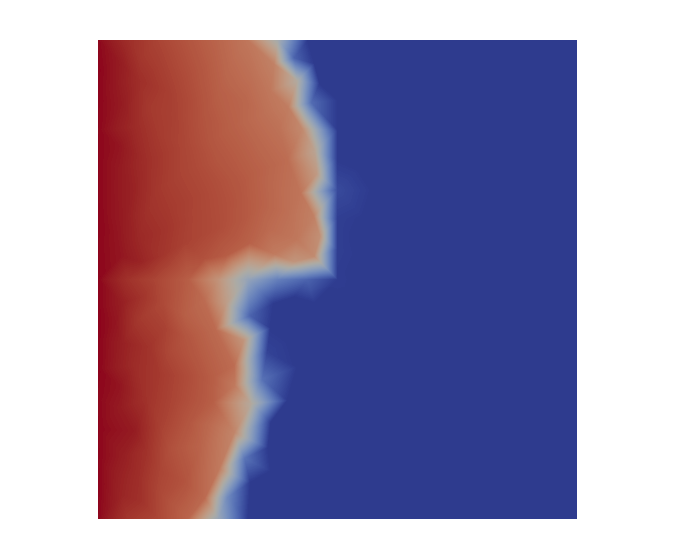
\includegraphics[width=.56\textwidth]{./Pics/SVDCase/SVDCase_Saturation_t_dot50.png}}
\vspace{0.cm}
\hbox{\hspace{0.5cm} (a) Phase 1 Saturation at t=0.15s \hspace{3.75cm} (b) t=0.30s \hspace{5.0cm} (c) t=0.50s}
\vspace{0.5cm}
\hbox{
      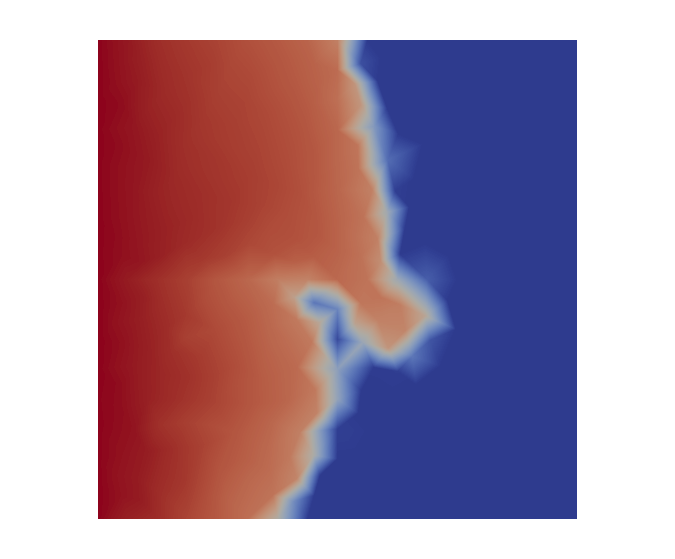
\includegraphics[width=.56\textwidth]{./Pics/SVDCase/SVDCase_Saturation_t_1dot15.png}
      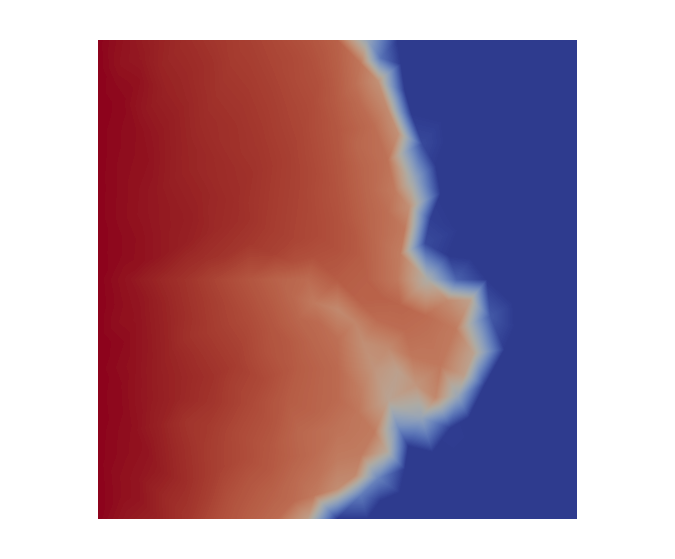
\includegraphics[width=.56\textwidth]{./Pics/SVDCase/SVDCase_Saturation_t_1dot75.png} 
      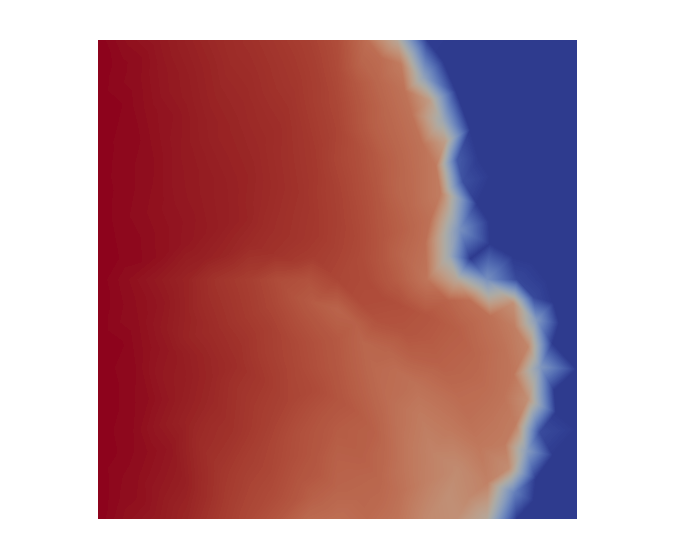
\includegraphics[width=.56\textwidth]{./Pics/SVDCase/SVDCase_Saturation_t_2dot95.png}}
\vspace{0.cm}
\hbox{ \hspace{2.5cm} (d) t=1.15s \hspace{5.5cm} (e) t=1.75s   \hspace{5.5cm} (f) t=2.95s}
\vspace{0.cm}
}   
\caption{Simulation for the SVDCase (Saturation legend in Fig.~\ref{fig:SVDCase_Saturation}(a) is representative for all the other figures - \ie Fig.~\ref{fig:SVDCase_Saturation}(b) to (f))}
\label{fig:SVDCase_Saturation}
\end{figure}
\end{landscape}
\clearpage



%%%%
%%%%  FIGURE
%%%%
\begin{landscape}
\begin{figure}[ht] 
\vbox{\vspace{-1cm}
\hspace{0.0cm} \hbox{\hspace{4cm} 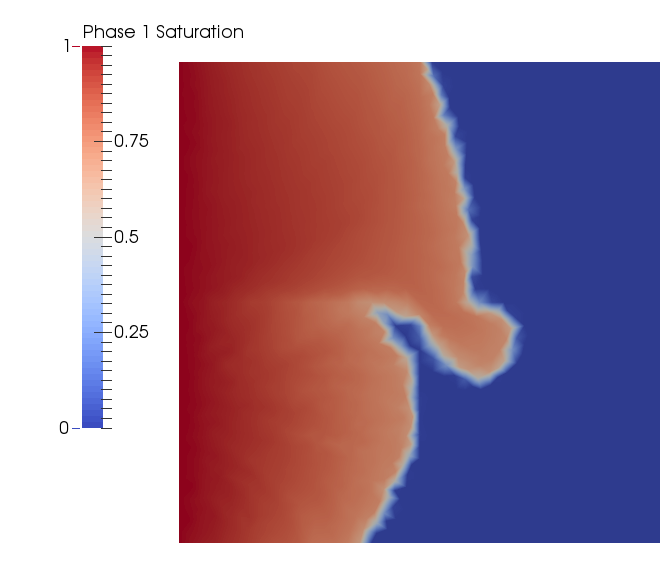
\includegraphics[width=.56\textwidth]{./Pics/BaseCase/BaseCase_Saturation_t_1dot15withlegend.png}
      \hspace {1.5cm} 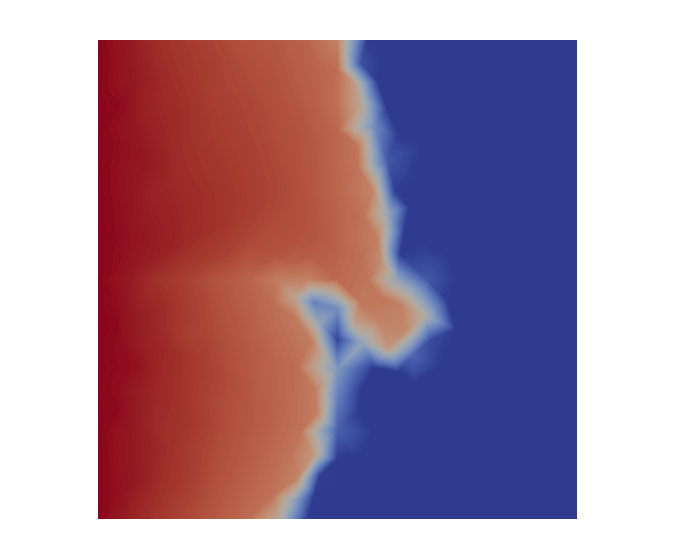
\includegraphics[width=.56\textwidth]{./Pics/ArithMeanCase/ArithMeanCase_Saturation_t_1dot15.png}}
\vspace{0.cm}
\hbox{\hspace{7.0cm} (a) BaseCase \hspace{5.75cm} (b) ArithMeanCase}
\vspace{0.5cm}
\hbox{
      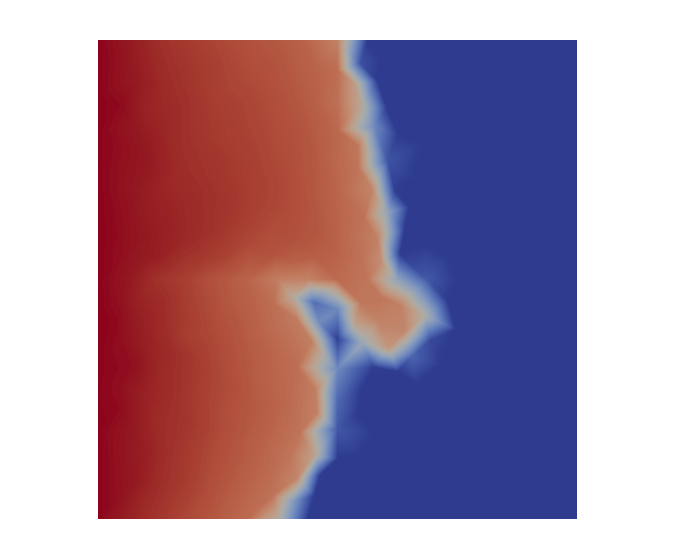
\includegraphics[width=.56\textwidth]{./Pics/HarmMeanCase/HarmMeanCase_Saturation_t_1dot15.png}
      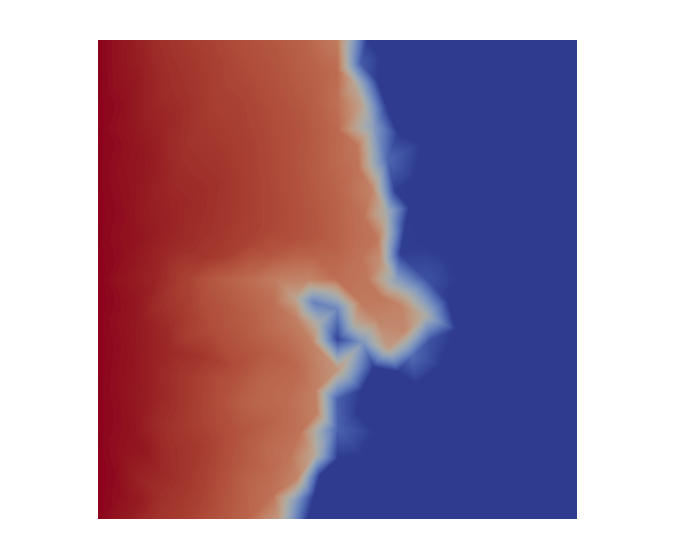
\includegraphics[width=.56\textwidth]{./Pics/PDFCase/PDFCase_Saturation_t_1dot15.png} 
      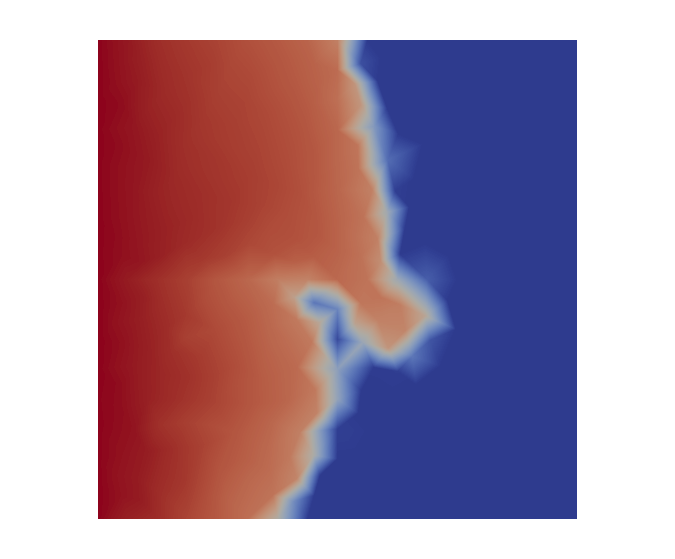
\includegraphics[width=.56\textwidth]{./Pics/SVDCase/SVDCase_Saturation_t_1dot15.png}}
\vspace{0.cm}
\hbox{ \hspace{1.75cm} (c) HarmMeanCase \hspace{5.0cm} (d) PDFCase \hspace{5.0cm} (e) SVDCase}
\vspace{0.cm}
}   
\caption{Comparing phase 1 saturation distribution for all the models at $t=1.15$ s (Saturation legend in Fig.~\ref{fig:Saturationfield@t=1.15s}(a) is representative for all the other figures - \ie Fig.~\ref{fig:Saturationfield@t=1.15s}(b) to (e))}
\label{fig:Saturationfield@t=1.15s}
\end{figure}
\end{landscape}
\clearpage

%%%%
%%%%  FIGURE
%%%%
%\begin{landscape}

%\begin{figure}[ht] 
%\vbox{\vspace{-1cm}
%\centering
%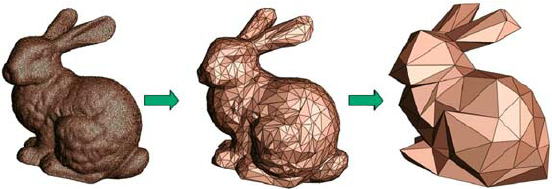
\includegraphics[width=.56\textwidth]{./Pics/Introduction/Graphical-illustration-of-model-order-reduction.png}
%\vspace{0.cm}
%\vspace{0.5cm}
%}   
%\caption{Graphical illustration of model order reduction (initially used by \citet{Schilders2008}, with graphics credited to Harvard University, Microsoft Research.)}
%\vspace{1.5cm}
%\label{fig:IllustrationMOR}
%\end{figure}

\begin{figure}[ht] 
\vbox{\vspace{-1cm}
\hbox{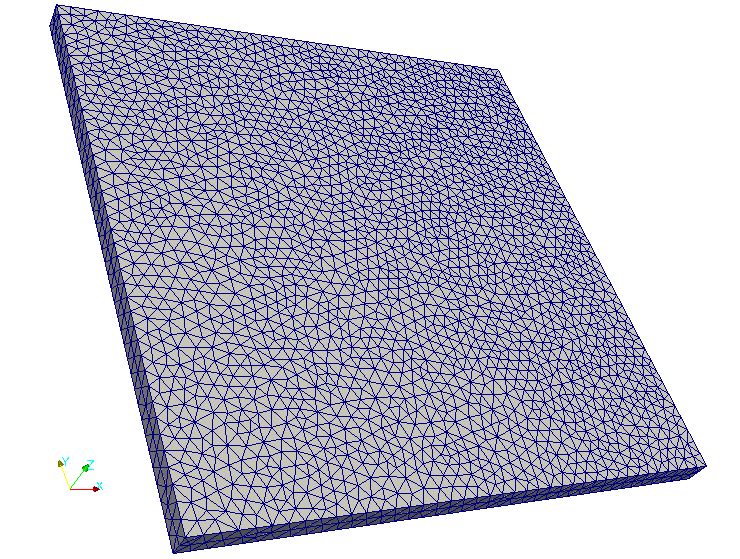
\includegraphics[width=.56\textwidth]{./Pics/3D_BaseCase/3D_BaseCase_MeshOnly.png}
      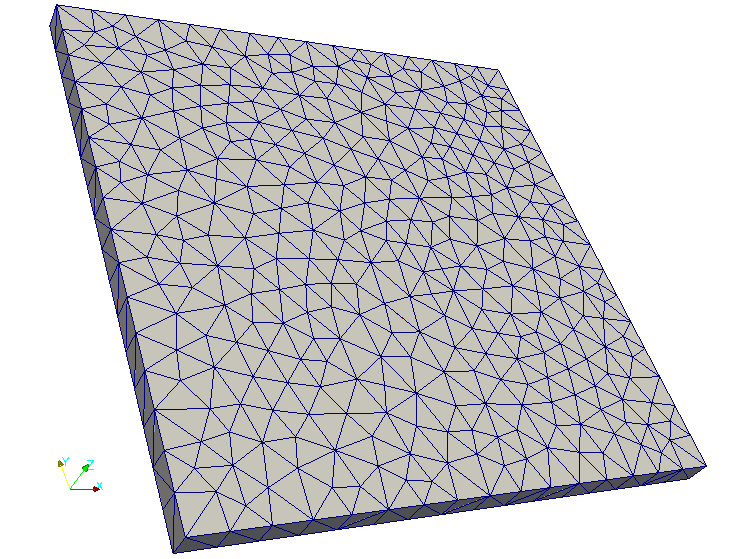
\includegraphics[width=.56\textwidth]{./Pics/3D_HOSVDCase/3D_HOSVDCase_MeshOnly.png}}
\vspace{0.cm}
\hbox{\hspace{0.05cm} (a) 3-D High Resolution Grid (BaseCase) \hspace{0.05cm} (b) 3-D Low Resolution Grid (Upscaled Cases) \hspace{3.0cm}}
\vspace{0.5cm}
}   
\caption{Mesh grid used in the performed numerical 3-D simulations: (a) high-resolution and (b) upscaled cases with 2019 and 303 tetrahedral elements respectively}
\label{fig:HiRes_LowRes_3D_Mesh}
\end{figure}


%\end{landscape}
\clearpage

%%%%
%%%%  FIGURE
%%%%
\begin{landscape}
\begin{figure}[ht] 
\vbox{\vspace{-1cm}
\hspace{0.0cm} \hbox{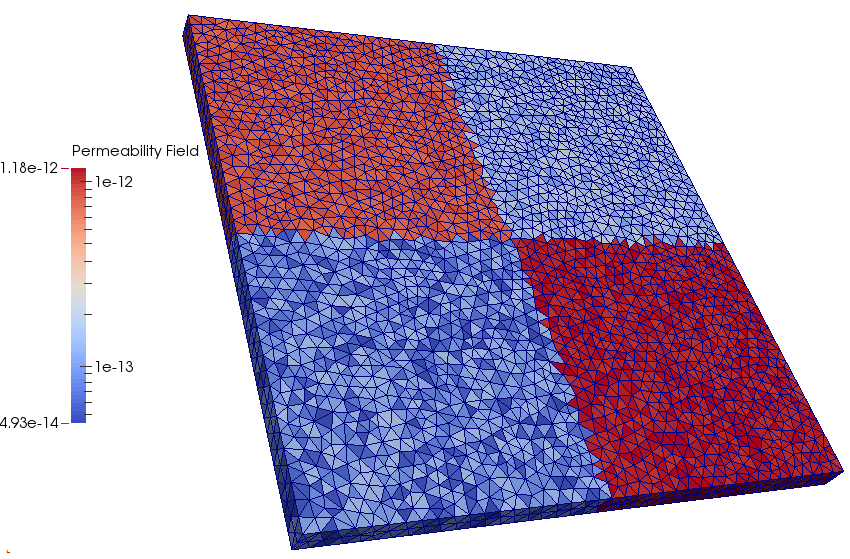
\includegraphics[width=.8\textwidth]{./Pics/3D_BaseCase/3D_BaseCase_PermField_withMesh2.png}
      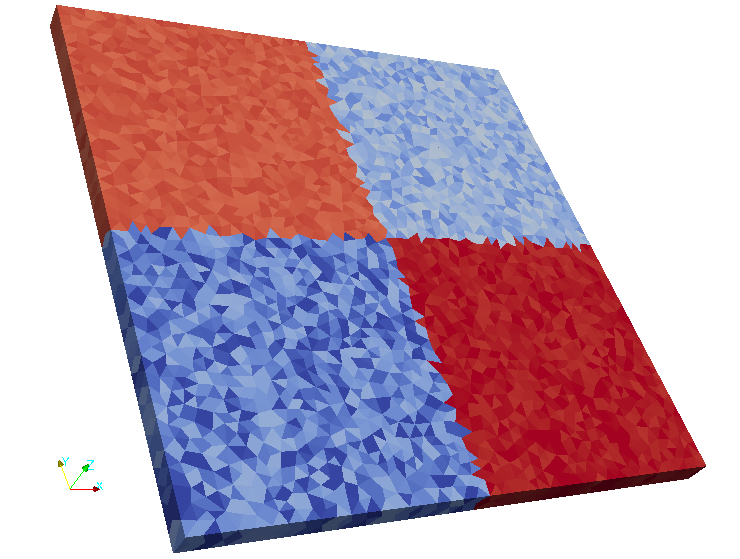
\includegraphics[width=.7\textwidth]{./Pics/3D_BaseCase/3D_BaseCase_PermField_withoutMesh.png}}
\vspace{0.cm}
\hbox{(a) 3-D BaseCase (overlapped with the mesh) \hspace{3.75cm} (b) 3-D BaseCase (without Mesh)}
\vspace{0.5cm}
\hbox{\includegraphics[width=.7\textwidth]{./Pics/3D_HOSVDCase/3D_HOSVDCase_PermField_withMesh.png}
      \includegraphics[width=.7\textwidth]{./Pics/3D_HOSVDCase/3D_HOSVDCase_PermField_withoutMesh.png}}
\vspace{0.cm}
\hbox{(c) 3-D HOSVD Case (overlapped with the mesh) \hspace{4.75cm} (d) 3-D HOSVD Case (without Mesh)}
\vspace{0.cm}
}   
\caption{Permeability field for the 3D base case as well as the HOSVD upscaled cases (Permeability legend in Fig.~\ref{fig:3D_PermFields}(a) is representative for all the other figures - \ie Fig.~\ref{fig:3D_PermFields}(b) to (d))}
\label{fig:3D_PermFields}
\end{figure}
\end{landscape}
\clearpage

%%%%
%%%%  FIGURE
%%%%
\begin{landscape}
\begin{figure}[ht] 
\vbox{\vspace{-1cm}
\hspace{0.0cm} \hbox{\includegraphics[width=.6\textwidth]{./Pics/3D_BaseCase/3D_BaseCase_Saturation_tdot18withMesh2.png}
      \includegraphics[width=.5\textwidth]{./Pics/3D_BaseCase/3D_BaseCase_Saturation_tdot28.png}
      \includegraphics[width=.5\textwidth]{./Pics/3D_BaseCase/3D_BaseCase_Saturation_tdot42.png}}
\vspace{0.cm}
\hbox{\hspace{0.5cm} (a) 3-D BaseCase at t=0.18s \hspace{1.0cm} (b) 3-D BaseCase at t=0.28s \hspace{3.0cm} (c) 3-D BaseCase at t=0.42s}
\vspace{0.5cm}
\hbox{
      \includegraphics[width=.5\textwidth]{./Pics/3D_HOSVDCase/3D_HOSVDCase_Saturation_tdot18withMesh.png}
      \includegraphics[width=.5\textwidth]{./Pics/3D_HOSVDCase/3D_HOSVDCase_Saturation_tdot28.png} 
      \includegraphics[width=.5\textwidth]{./Pics/3D_HOSVDCase/3D_HOSVDCase_Saturation_tdot42.png}}
\vspace{0.cm}
\hbox{ \hspace{1.5cm} (d) HOSVD Case at t=0.18s \hspace{1.0cm} (e) HOSVD Case at t=0.28s  \hspace{3.0cm} (f) HOSVD Case at t=0.42s}
\vspace{0.cm}
}   
\caption{Comparing phase 1 saturation distribution for the 3-D Cases at $t=0.18, 0.28$ and $0.42$ s (Saturation legend in Fig.~\ref{fig:Saturationfield4_3DCases}(a) is representative for all the other figures - \ie Fig.~\ref{fig:Saturationfield4_3DCases}(b) to (e))}
\label{fig:Saturationfield4_3DCases}
\end{figure}
\end{landscape}
\clearpage


